\hypertarget{entropy}{%
\subsection{Entropy}\label{entropy}}

You may recall from high school physics that entropy has something to do
with thermodynamics. Why in the world is it used to describe passwords?

Claude Shannon coined the use of the term entropy in information theory
when he recognized the formula he had developed for measuring
information also occurred in statistical mechanics, where it was called
entropy! He used the letter H to represent it since it was so in
Boltzmann's famous H theorem, which has to do with molecules moving to
equilibrium.

\begin{wrapfigure}{i}{1.425in}
\vspace{-8pt}
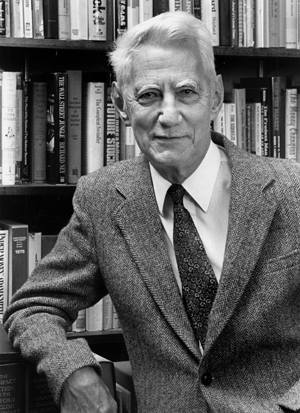
\includegraphics[width=1.425in,height=1.96181in]{./05_authentication/01_passwords/30_entropy/media/image1.jpeg}
\caption{Claude Shannon}
\end{wrapfigure}
For
passwords entropy denotes the uncertainty in the value of a password.
Entropy of passwords is conventionally expressed in bits, which brings
you back to high school math. That's right logarithms! If your alphabet
consists of 26 letters, say and you require 8 letters in your password
then there are 26\textsuperscript{8} possible passwords. That can be
expressed as entropy with

H = log\textsubscript{2}(26\textsuperscript{8}) = 37.6 bits

More information is provided by NIST at
\url{https://pages.nist.gov/800-63-3/sp800-63b.html}

Humans don't do random very well, so in reality, much of the possible
space is never taken by self-selected passwords, so in practice the
entropy is overstates the value.

Of course, modern computers with access to the password hash file can
make quick work of this. So finding ways to prevent or throttle password
guessing is important! Or, better yet, don't rely entirely on passwords!
